\documentclass{beamer}
\usepackage{booktabs}
\usepackage{graphicx}
\usepackage{amsmath}
\usepackage{array}
\usetheme{default}
\setbeamertemplate{navigation symbols}{}
\setbeamertemplate{footline}{\hfill\insertframenumber/\inserttotalframenumber\hspace{1.5em}}

\title{Robust Constraint Learning: Research Update}
\subtitle{Formulation, Calibration, Evaluation}
\date{\today}

\begin{document}

\begin{frame}
  \titlepage
\end{frame}

% ===========================================================================
\begin{frame}{Formulation}
  \textbf{Nominal}:
  \[
    \min_{x\in\mathcal{X}}\; c^\top x \quad\text{s.t.}\quad \hat f(x;\theta^\ast)\le b .
  \]
  \begin{itemize}
    \item Noisy labels $\Rightarrow$ different $\theta^\ast(\delta)$ $\Rightarrow$ infeasible
      decisions.
    \item \textbf{Robust}: feasible against \emph{every} reachable model.
  \end{itemize}
  \[
    \min_{x\in\mathcal{X}} c^\top x
    \;\;\text{s.t.}\;\; \max_{\delta\in\mathcal{D}} f(x;\theta^\ast(\delta))\le b,
    \quad \theta^\ast(\delta)=\arg\min_{\theta\in\Theta_{\text{feas}}}\mathcal L(\theta;X,y+\delta)
  \]
\end{frame}

% ===========================================================================
\begin{frame}{Problem settings: synthetic}
  True constraint, known exactly (evaluation only):
  \[
    f_{\text{true}}(x) = \sum_{j=1}^d x_j^2 + 0.5\prod_{j=1}^d x_j, \qquad x\in[0,1]^d
  \]
  Noisy labels $y_i = f_{\text{true}}(x_i)+\varepsilon_i$,
  $\varepsilon_i\sim\mathcal N(0,\sigma^2)$:
  \[
    \min_{x\in[0,1]^d} \; -\sum_{j=1}^d x_j \quad\text{s.t.}\quad \hat f(x;\theta)\le b,
    \qquad b=0.5\,d
  \]
  \begin{itemize}
    \item One LP, one learned constraint, no context.
  \end{itemize}
\end{frame}

\begin{frame}{Problem settings: gastric}
  \small
  \textbf{A row is a published trial arm.} Meta-analysis of gastric-cancer
  chemotherapy studies; $z$, $x$ and the labels are all arm-level \emph{aggregates}.
  \begin{itemize}
    \item \textbf{416 arms}, split by publication year:
      \textbf{320 train} ($\le$ 2008) / \textbf{96 test} (2009--2012).
    \item $x$: drug doses, in the hull of observed arms; one LP per arm.
    \item $y$: \% of the arm with grade-3/4 toxicity, per category; median OS.
    \item All 6 models are fit on the \emph{same} 320 arms $\Rightarrow$ one relabeling
      $\delta$ moves them together. \textbf{Coherent} relabeling uses that one shared draw across all constraints;
      a private $\delta_c$ per constraint can also be done.
  \end{itemize}
  \[
    \max_{x\,\in\,\mathrm{hull}(X_\text{train})} \widehat{\text{OS}}(x,z;\theta_\text{os})
    \quad\text{s.t.}\quad \widehat{\text{pctl}}_c(x,z;\theta_c) \le 0.6
  \]
  \[
    c\in\{\text{DLT, Blood, Constitutional, Infection, GI}\}
  \]
  \textbf{$z$ --- 9 arm-level covariates}, fixed within an arm:
  \begin{center}\footnotesize
  \begin{tabular}{@{}lll@{}}
    \texttt{Pub\_Year} & \texttt{FRAC\_MALE} & \texttt{Primary\_Stomach} \\
    \texttt{Asia} & \texttt{AGE\_MED} & \texttt{Primary\_GEJ} \\
    \texttt{N\_Patient} & \texttt{Prior\_Palliative\_Chemo} & \texttt{ECOG\_MEAN} \\
  \end{tabular}
  \end{center}
  \footnotesize
  All \emph{fractions of the arm} except \texttt{Pub\_Year}, \texttt{N\_Patient}
  (11--521), \texttt{AGE\_MED} (yrs), \texttt{ECOG\_MEAN} (grade 0--4).
\end{frame}

% ---------------------------------------------------------------------------
\begin{frame}{Problem settings: comparison}
  \small
  \begin{center}
  \begin{tabular}{@{}>{\raggedright\arraybackslash}p{3.4cm}>{\raggedright\arraybackslash}p{3.4cm}>{\raggedright\arraybackslash}p{3.9cm}@{}}
    \toprule
    & Synthetic & Gastric \\
    \midrule
    Constraints / LP & 1 & 5 + objective \\
    LPs at evaluation & 1 & many (one per arm) \\
    Coherence & vacuous & \textbf{binding}: 6 models, one set of arms \\
    \bottomrule
  \end{tabular}
  \end{center}
\end{frame}

% ---------------------------------------------------------------------------
\begin{frame}{Model class is chosen \emph{once}, before any robustness}
  \small
  5-fold CV on the \textbf{training} split; grid over
  \{linear (ElasticNet), SVM, CART, RF, GBM, XGB, MLP\}; score $=R^2$.
  \begin{itemize}
    \item Winner (type \emph{and} hyperparameters) frozen per learned model
      (5 constraints + OS).
    \item Gastric: XGB for DLT / Blood / Constitutional / Infection; ElasticNet for GI and OS.
    \item Ensures the model is \emph{fixed} across all robustness methods and does not confound.
  \end{itemize}
\end{frame}

% ===========================================================================
\begin{frame}{Robust methods: overview}
  Shared MIP scaffolding --- they differ in \emph{where} robustness enters.
  \begin{itemize}
    \item \textbf{Nominal} --- none.
    \item \textbf{Robust Regression} --- one label-robust model per constraint.
    \item \textbf{Wrapper} --- chance constraint over $P$ bootstrap models.
    \item \textbf{Cutting Planes (ours)} --- cut worst-case models near $x^\ast$.
    \item Each robustness method has a single knob to sweep for a Pareto frontier.
  \end{itemize}
\end{frame}

% ---------------------------------------------------------------------------
\begin{frame}{Robust Regression --- one label-robust model per constraint}
  \[
    \min_\theta \max_{\delta\in\mathcal D} \mathcal L(\theta; X, y+\delta), \qquad
    \mathcal D = \{\delta : |\delta_i|\le\varepsilon,\ \lVert\delta\rVert_1\le\gamma\}
  \]
  \begin{itemize}
    \item \textbf{Knob}: $\varepsilon = \texttt{label\_eps}\cdot\mathrm{sd}(y)$ ---
      $\texttt{label\_eps}$ is unitless, so one grid covers toxicity fractions and OS months.
    \item $\gamma = \texttt{budget\_frac}\cdot n\,\varepsilon$ --- $\texttt{budget\_frac}$
    held fixed at 0.5, n=number of train points.
    \item \textbf{Linear}: exact QP, solved once (next slide).
    \item \textbf{Trees / ensembles}: no closed form --- alternate worst $\delta$ /
      retrain, $K$ times.
    \item \textbf{Not coherent}: solved per constraint, so each constraint gets its own
      $\delta_c$.
  \end{itemize}
\end{frame}

\begin{frame}{Robust Regression: the linear counterpart is an exact QP}
  \small
  Inner max over $\mathcal D$ is attained at a vertex --- shift the $m$ largest
  residuals by $\varepsilon$ in their own sign:
  \[
    \max_{\delta\in\mathcal D}\lVert r+\delta\rVert^2
      = \lVert r\rVert^2 + 2\varepsilon\, S_m(|r|) + m\varepsilon^2,
    \qquad r = y - Z\beta - b_0,
  \]
  with $S_m$ = sum of the $m$ largest $|r_i|$ (convex, LP-representable; the
  $m\varepsilon^2$ is constant in $\theta$ and dropped). So
  \[
  \begin{aligned}
    \min_{\beta,b_0,r,a,q,t}\;\; & \tfrac{1}{2n}\Big[\textstyle\sum_i r_i^2
      + 2\varepsilon\big(m\,t + \sum_i q_i\big)\Big]
      + \alpha\lambda\lVert\beta\rVert_1
      + \tfrac{\alpha}{2}(1-\lambda)\lVert\beta\rVert_2^2 \\
    \text{s.t.}\;\; & r_i = y_i - \beta^\top z_i - b_0, \quad i=1..n \\
                    & a_i \ge r_i,\quad a_i \ge -r_i, \quad
                      q_i \ge a_i - t, \quad q_i \ge 0
  \end{aligned}
  \]
  \begin{itemize}
    \item $m\,t+\sum_i q_i$ is the LP epigraph of $S_m(|r|)$ at the optimum.
    \item Penalty matches sklearn's ElasticNet scaling $\Rightarrow$ directly comparable
      to the nominal fit; $\varepsilon=0$ recovers it.
  \end{itemize}
\end{frame}

\begin{frame}{Wrapper}
  \begin{itemize}
    \item $P$ bootstrap resamples; $P$ replicates of each learned model, all embedded.
    \item $z_p=1$ iff $x$ satisfies \emph{every} constraint under replicate $p$
      $\Rightarrow$ \textbf{coherent} (one draw per replicate).
    \item Chance constraint: $\tfrac1P\sum_p z_p \ge 1-\alpha$.
    \item OS: worst-case epigraph over the same replicates.
    \item Knob: $\alpha$.
  \end{itemize}
\end{frame}

\begin{frame}{Cutting Planes (ours)}
  \small
  \begin{enumerate}
    \item Solve master $\to x^\ast$ --- gastric: the \emph{shared} master once per
      \textbf{anchor} (10 k-medoids over \emph{training} contexts) $\to x^\ast_1..x^\ast_{10}$.
    \item \textbf{Separate}: resample near $x^\ast$, retrain, take the worst model
      (next slide).
    \item Cut if violation $>$ tolerance.
  \end{enumerate}
  \begin{itemize}
    \item \textbf{basic} (synthetic): retrain the 20 resamples, score at $x^\ast$,
      cut the single worst (coherence vacuous --- one constraint).
    \item \textbf{coherent} (gastric): one shared relabeling trains all 5 constraints
      \emph{and} the objective; rank scenarios by mean exceedance over
      (anchor $\times$ learned model), cut the worst \emph{scenario}.
    \item One cut, fully embedded, valid at \emph{any} context $\Rightarrow$ cuts computed
      \textbf{offline}; test points enter only at prescribe time (re-solve, context pinned).
    \item \textbf{OS robustification off by default \emph{in CP}} --- ablation: worse test
      feasibility \emph{and} OS. (Wrapper always robustifies OS; no toggle.)
  \end{itemize}
\end{frame}

\begin{frame}{Cutting Planes: the localized resample}
  \small
  \textbf{Pool} --- $k$ nearest training rows to $x^\ast$, Euclidean in
  \emph{standardized} features; \texttt{distance=full} (context + decision).
  Gastric: \emph{union} of the $k$-NN sets over all 10 anchors.
  \medskip

  \textbf{Scenario} --- draw $n$ indices \emph{with replacement from the pool}:
  full-size training set, local rows oversampled, distant rows absent.
  Retrain with the \emph{actual} model type.
  20 scenarios / iteration, $\le$ 20 iterations.
  \medskip

  \textbf{$k=\min(n,\max(100,\,0.1n))$ --- the floor binds in both problems}
  \begin{itemize}
    \item Min 100 ensures we have enough unique data points to train models.
    \item Gastric $100/320$; synthetic $100/200$ = \emph{half} the data.
    \item \textbf{Gastric}: Union over anchors grows it further: logged \texttt{PoolFrac} $=0.39$.
    \item $\Rightarrow$ localization weaker than intended, and
      \texttt{k\_neighbors\_frac} is inert. Lower the floor to make it live.
  \end{itemize}
\end{frame}

\begin{frame}{Cutting Planes: knobs}
  \textbf{$\tau$ --- stopping tolerance} (the robustness dial)
  \begin{itemize}
    \item Dimensionless: \texttt{tolerance} $=\tau\cdot d_0$.
    \item $d_0$ = iteration-0 worst violation; measured once.
    \item $\tau=1\equiv$ nominal; $\tau\to 0$ cuts maximally.
    \item Relative $\Rightarrow$ one grid transfers ($d_0\!\approx\!0.01$ vs.\ $0.45$).
  \end{itemize}
  \medskip
  \textbf{Coverage}
  \begin{itemize}
    \item Adding cuts may make the MIP infeasible.
    \item Add a rule where if the MIP becomes infeasible, either roll back the cut, or admit them by evicting a stale cut (slack at $x^*$).
  \end{itemize}
\end{frame}

\begin{frame}{Cutting Planes: open questions}
  \textbf{1. In step 2, retrain with a localized bootstrap, or an assumed noise distribution?}
  \begin{itemize}
    \item Now: localized bootstrap --- data-driven, spread pinned to $n$.
    \item Well-specified on synthetic, but not on gastric.
    \item Sharing Robust Reg.'s $\mathcal D$ isolates decision- vs model-robustness.
  \end{itemize}
  \medskip
  \textbf{2. Cutting planes per test point, or once over all anchors?}
  \begin{itemize}
    \item Per test point (n=96): tailored --- but many different LPs.
    \item Over train anchors (now): offline --- but $x^\ast_1..x^\ast_{10}$ may not represent test points.
  \end{itemize}
\end{frame}

% ===========================================================================
\begin{frame}{Robustness Calibration: one knob each, \texttt{label\_eps} / $\tau$}
  So that the different methods are comparable, we tune their robustness knobs.
  Write $\kappa$ for a method's knob generically ($\varepsilon$ for Robust Reg., $\tau$ for CP).
  \medskip

  \textbf{Held-out CV}
  \begin{itemize}
    \item $\kappa^\ast$ = max feasibility s.t.\ objective within budget.
    \item Scored using a GT ensemble fit on train only.
    \item Gastric: temporal forward-chaining folds; synthetic: KFold.
    \item Gives $\varepsilon^\ast=0.10$ (Robust Reg.) and $\tau^\ast=0.10$ (CP).
  \end{itemize}
\end{frame}

% ===========================================================================
\begin{frame}{Evaluation}
  \small
  \begin{center}
  \begin{tabular}{@{}>{\raggedright\arraybackslash}p{2.6cm}>{\raggedright\arraybackslash}p{4.0cm}>{\raggedright\arraybackslash}p{4.0cm}@{}}
    \toprule
    & Gastric & Synthetic \\
    \midrule
    Ground truth & GT ensemble, fit on all \textbf{416} arms (train + test) & Exact analytic constraint \\[0.3em]
    New train draw & $m$ of $n=320$ arms, no replacement
      ($m=160$ at frac 0.5, $256$ at 0.8); 30 draws headline, 10 in sweeps
      & Regenerate fresh noise \\
    \bottomrule
  \end{tabular}
  \end{center}
  \begin{itemize}
    \item \textbf{A single draw using all training data favours nominal}: GT is fit on a
      \emph{superset} of the constraint models' rows, so we subsample instead.
  \end{itemize}
  \medskip
  \footnotesize
  \textbf{Samestore cohort} (gastric) --- every reported number, \emph{feasibility and
  OS alike}, is a mean over the test arms that \textbf{every} method could prescribe
  for (in the Pareto sweep, every method $\times$ strength cell). Recomputed
  \emph{per draw}: 83--96 of 96 arms (all-constr., mean 93), 93--96 (DLT).
  $\Rightarrow$ feasibility is \textbf{conditional on solvability}, which is therefore
  reported separately.
\end{frame}

% ===========================================================================
\begin{frame}{Synthetic noise sweep --- at fixed robustness knobs}
  \centering
  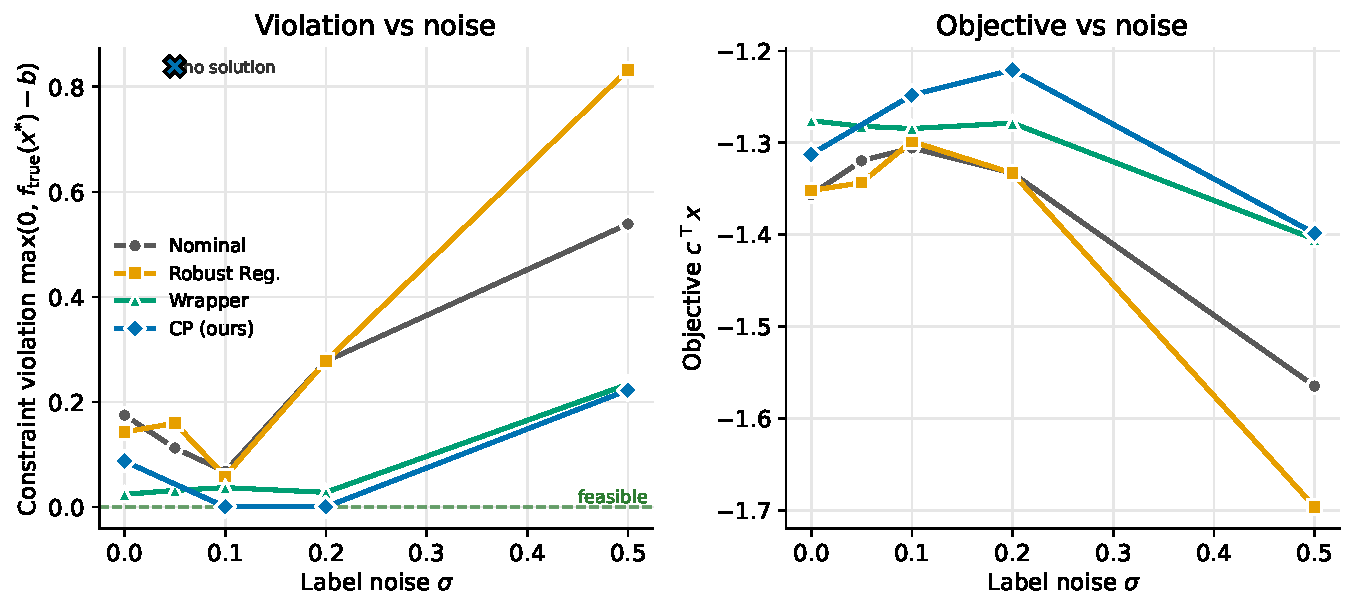
\includegraphics[width=0.85\linewidth]{../results/figures/fig_synthetic.pdf}

  \raggedright\small
  \begin{itemize}
    \item We change the noise added to the training labels.
    \item CP is the only method to achieve zero violation, but it has the worst objective.
    \item Need to re-run with CV-tuned robustness knobs.
  \end{itemize}
\end{frame}

\begin{frame}{Gastric results (CV-calibrated robustness)}
  \centering
  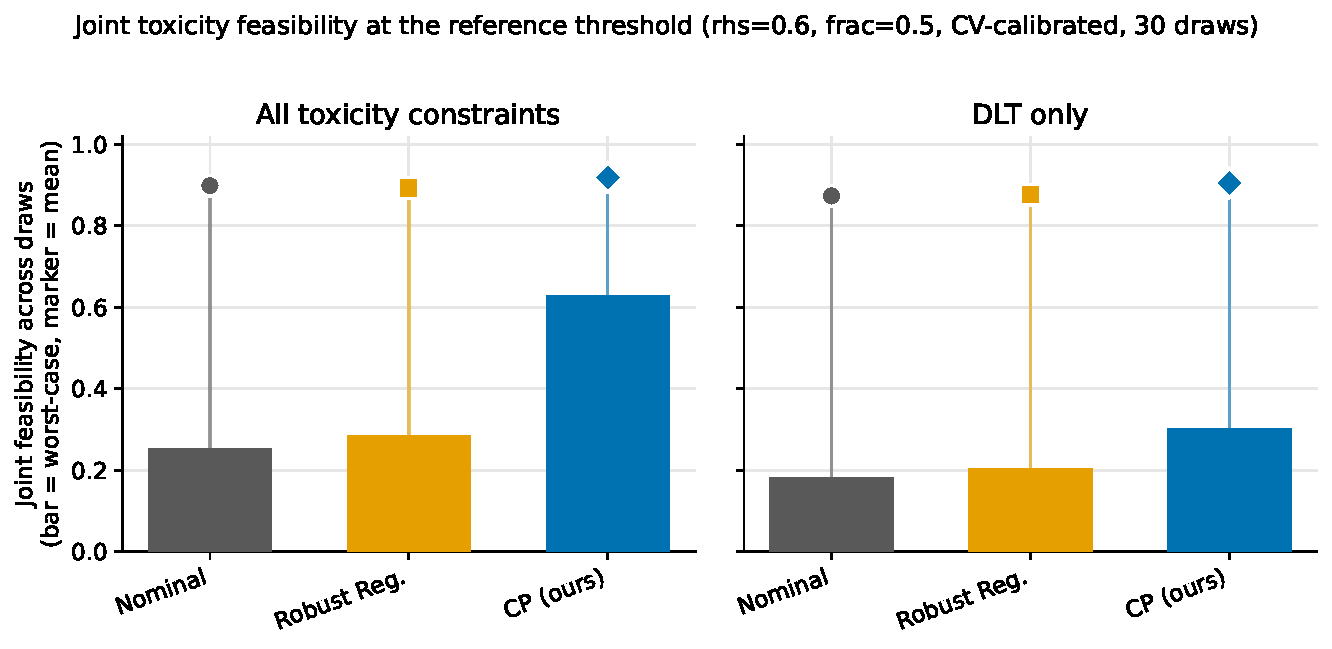
\includegraphics[width=0.76\linewidth]{../results/figures/fig_headline.pdf}

  \raggedright\footnotesize
  \begin{itemize}
    \item $\kappa^\ast$ from CV, rhs$=0.6$, subsample frac$=0.5$, 30 draws.
      Worst-case feasibility (nom / RR / CP):
    \item all-constraints \; 0.25 / 0.28 / \textbf{0.63} \hspace{1.2em}
      DLT-only \; 0.18 / 0.20 / \textbf{0.30}
    \item Similar mean feasibility, but CP has better worst-case feasibility.
    \item Evaluated on arms that were solvable across all methods
          (sometimes the MIP would become infeasible, so we couldn't generate an $x^*$ to
          evaluate GT feasibility).
    \item Wrapper excluded: too slow.
  \end{itemize}
\end{frame}

\begin{frame}{Gastric results: objective vs.\ worst-case feasibility}
  \centering
  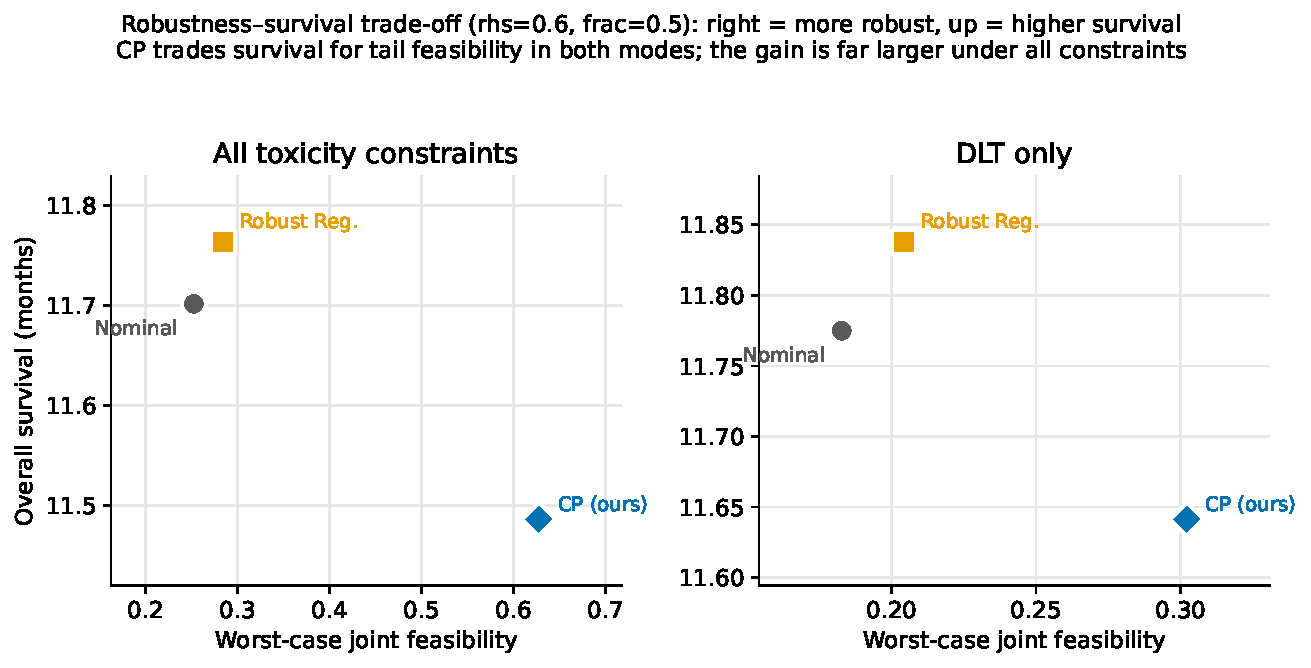
\includegraphics[width=0.9\linewidth]{../results/figures/fig_tradeoff.pdf}

  \raggedright\footnotesize
  \begin{itemize}
    \item Previous slide showed that CP is more robust, but it also has a worse objective (OS) than the other methods.
    \item Next we sweep the knobs to see if we can find a better trade-off between objective and feasibility for all methods.
  \end{itemize}
\end{frame}

% ===========================================================================
\begin{frame}{Summary}
  \small
  \textbf{Methodology}
  \begin{enumerate}
    \item \textbf{Fix the model class first.} CV picks type + hyperparameters,
    then freezes them so model choice can't confound the comparison.
    \item \textbf{Robustify.} Shared MIP scaffolding; methods differ only in
      \emph{where} robustness enters, each via a single monotone knob.
    \item \textbf{Calibrate the knob.} Held-out CV picks $\kappa^\ast$ = max
      feasibility s.t.\ an objective budget $\Rightarrow$ matched robustness level.
    \item \textbf{Evaluate against a fixed ground truth.} Repeated subsampled
      training draws, scored out-of-sample by the GT ensemble (synthetic: the exact
      constraint), on the cohort every method could prescribe for.
  \end{enumerate}
  \medskip
  \textbf{Findings}
  \begin{itemize}
    \item CP gives the best \emph{worst-case} feasibility at CV-calibrated knobs,
      at the cost of a worse objective (OS).
    \item To improve the trade-off, we need to sweep the robustness knobs for all methods.
  \end{itemize}
\end{frame}

\begin{frame}{Next steps}
  \textbf{Method}
  \begin{itemize}
    \item CP: sample from a noise distribution rather
      than a bootstrap, for gastric \emph{and} synthetic --- bootstrapping is
      unreliable at these sample sizes.
    \item Coherent Robust Regression.
  \end{itemize}
  \medskip
  \textbf{Experiments \& reporting}
  \begin{itemize}
    \item Run synthetic over multiple draws with CV-tuned knobs.
    \item Robustness sweeps for both synthetic and gastric.
    \item Remove OS robustification from the wrapper for a fair comparison.
    \item Fix DLT-only plots --- evaluate DLT-only feasibility, not joint.
    \item Add WFP problem setting.
  \end{itemize}
\end{frame}

\end{document}
